%!TEX TS-program = pdflatexmk
\documentclass[12pt]{article}
%\IEEEoverridecommandlockouts
% The preceding line is only needed to identify funding in the first footnote. If that is unneeded, please comment it out.
\usepackage{cite}
\usepackage{amsmath,amssymb,amsfonts}
\usepackage{algorithmic}
% \usepackage{subcaption}
\usepackage{graphicx}
\usepackage{hyperref}
\usepackage{textcomp}
\usepackage{xurl}
\usepackage{xcolor}
\usepackage{array}
\usepackage{tabu}
\usepackage{float}

\def\BibTeX{{\rm B\kern-.05em{\sc i\kern-.025em b}\kern-.08em
    T\kern-.1667em\lower.7ex\hbox{E}\kern-.125emX}}

\DeclareRobustCommand*{\IEEEauthorrefmark}[1]{%
  \raisebox{0pt}[0pt][0pt]{\textsuperscript{\footnotesize #1}}%
}

%\usepackage{amsmath,amsthm,amscd,amssymb}
\usepackage[noBBpl,sc]{mathpazo}
\usepackage[papersize={6.8in, 10.0in}, left=.5in, right=.5in, top=.6in, bottom=.9in]{geometry}
\linespread{1.1}
\sloppy
\raggedbottom
\pagestyle{plain}

% these include amsmath and that can cause trouble in older docs.
\makeatletter
\@ifpackageloaded{amsmath}{}{\RequirePackage{amsmath}}

\DeclareFontFamily{U}  {cmex}{}
\DeclareSymbolFont{Csymbols}       {U}  {cmex}{m}{n}
\DeclareFontShape{U}{cmex}{m}{n}{
    <-6>  cmex5
   <6-7>  cmex6
   <7-8>  cmex6
   <8-9>  cmex7
   <9-10> cmex8
  <10-12> cmex9
  <12->   cmex10}{}

\def\Set@Mn@Sym#1{\@tempcnta #1\relax}
\def\Next@Mn@Sym{\advance\@tempcnta 1\relax}
\def\Prev@Mn@Sym{\advance\@tempcnta-1\relax}
\def\@Decl@Mn@Sym#1#2#3#4{\DeclareMathSymbol{#2}{#3}{#4}{#1}}
\def\Decl@Mn@Sym#1#2#3{%
  \if\relax\noexpand#1%
    \let#1\undefined
  \fi
  \expandafter\@Decl@Mn@Sym\expandafter{\the\@tempcnta}{#1}{#3}{#2}%
  \Next@Mn@Sym}
\def\Decl@Mn@Alias#1#2#3{\Prev@Mn@Sym\Decl@Mn@Sym{#1}{#2}{#3}}
\let\Decl@Mn@Char\Decl@Mn@Sym
\def\Decl@Mn@Op#1#2#3{\def#1{\DOTSB#3\slimits@}}
\def\Decl@Mn@Int#1#2#3{\def#1{\DOTSI#3\ilimits@}}

\let\sum\undefined
\DeclareMathSymbol{\tsum}{\mathop}{Csymbols}{"50}
\DeclareMathSymbol{\dsum}{\mathop}{Csymbols}{"51}

\Decl@Mn@Op\sum\dsum\tsum

\makeatother

\makeatletter
\@ifpackageloaded{amsmath}{}{\RequirePackage{amsmath}}

\DeclareFontFamily{OMX}{MnSymbolE}{}
\DeclareSymbolFont{largesymbolsX}{OMX}{MnSymbolE}{m}{n}
\DeclareFontShape{OMX}{MnSymbolE}{m}{n}{
    <-6>  MnSymbolE5
   <6-7>  MnSymbolE6
   <7-8>  MnSymbolE7
   <8-9>  MnSymbolE8
   <9-10> MnSymbolE9
  <10-12> MnSymbolE10
  <12->   MnSymbolE12}{}

\DeclareMathSymbol{\downbrace}    {\mathord}{largesymbolsX}{'251}
\DeclareMathSymbol{\downbraceg}   {\mathord}{largesymbolsX}{'252}
\DeclareMathSymbol{\downbracegg}  {\mathord}{largesymbolsX}{'253}
\DeclareMathSymbol{\downbraceggg} {\mathord}{largesymbolsX}{'254}
\DeclareMathSymbol{\downbracegggg}{\mathord}{largesymbolsX}{'255}
\DeclareMathSymbol{\upbrace}      {\mathord}{largesymbolsX}{'256}
\DeclareMathSymbol{\upbraceg}     {\mathord}{largesymbolsX}{'257}
\DeclareMathSymbol{\upbracegg}    {\mathord}{largesymbolsX}{'260}
\DeclareMathSymbol{\upbraceggg}   {\mathord}{largesymbolsX}{'261}
\DeclareMathSymbol{\upbracegggg}  {\mathord}{largesymbolsX}{'262}
\DeclareMathSymbol{\braceld}      {\mathord}{largesymbolsX}{'263}
\DeclareMathSymbol{\bracelu}      {\mathord}{largesymbolsX}{'264}
\DeclareMathSymbol{\bracerd}      {\mathord}{largesymbolsX}{'265}
\DeclareMathSymbol{\braceru}      {\mathord}{largesymbolsX}{'266}
\DeclareMathSymbol{\bracemd}      {\mathord}{largesymbolsX}{'267}
\DeclareMathSymbol{\bracemu}      {\mathord}{largesymbolsX}{'270}
\DeclareMathSymbol{\bracemid}     {\mathord}{largesymbolsX}{'271}

\def\horiz@expandable#1#2#3#4#5#6#7#8{%
  \@mathmeasure\z@#7{#8}%
  \@tempdima=\wd\z@
  \@mathmeasure\z@#7{#1}%
  \ifdim\noexpand\wd\z@>\@tempdima
    $\m@th#7#1$%
  \else
    \@mathmeasure\z@#7{#2}%
    \ifdim\noexpand\wd\z@>\@tempdima
      $\m@th#7#2$%
    \else
      \@mathmeasure\z@#7{#3}%
      \ifdim\noexpand\wd\z@>\@tempdima
        $\m@th#7#3$%
      \else
        \@mathmeasure\z@#7{#4}%
        \ifdim\noexpand\wd\z@>\@tempdima
          $\m@th#7#4$%
        \else
          \@mathmeasure\z@#7{#5}%
          \ifdim\noexpand\wd\z@>\@tempdima
            $\m@th#7#5$%
          \else
           #6#7%
          \fi
        \fi
      \fi
    \fi
  \fi}

\def\overbrace@expandable#1#2#3{\vbox{\m@th\ialign{##\crcr
  #1#2{#3}\crcr\noalign{\kern2\p@\nointerlineskip}%
  $\m@th\hfil#2#3\hfil$\crcr}}}
\def\underbrace@expandable#1#2#3{\vtop{\m@th\ialign{##\crcr
  $\m@th\hfil#2#3\hfil$\crcr
  \noalign{\kern2\p@\nointerlineskip}%
  #1#2{#3}\crcr}}}

\def\overbrace@#1#2#3{\vbox{\m@th\ialign{##\crcr
  #1#2\crcr\noalign{\kern2\p@\nointerlineskip}%
  $\m@th\hfil#2#3\hfil$\crcr}}}
\def\underbrace@#1#2#3{\vtop{\m@th\ialign{##\crcr
  $\m@th\hfil#2#3\hfil$\crcr
  \noalign{\kern2\p@\nointerlineskip}%
  #1#2\crcr}}}

\def\bracefill@#1#2#3#4#5{$\m@th#5#1\leaders\hbox{$#4$}\hfill#2\leaders\hbox{$#4$}\hfill#3$}

\def\downbracefill@{\bracefill@\braceld\bracemd\bracerd\bracemid}
\def\upbracefill@{\bracefill@\bracelu\bracemu\braceru\bracemid}

\DeclareRobustCommand{\downbracefill}{\downbracefill@\textstyle}
\DeclareRobustCommand{\upbracefill}{\upbracefill@\textstyle}

\def\upbrace@expandable{%
  \horiz@expandable
    \upbrace
    \upbraceg
    \upbracegg
    \upbraceggg
    \upbracegggg
    \upbracefill@}
\def\downbrace@expandable{%
  \horiz@expandable
    \downbrace
    \downbraceg
    \downbracegg
    \downbraceggg
    \downbracegggg
    \downbracefill@}

\DeclareRobustCommand{\overbrace}[1]{\mathop{\mathpalette{\overbrace@expandable\downbrace@expandable}{#1}}\limits}
\DeclareRobustCommand{\underbrace}[1]{\mathop{\mathpalette{\underbrace@expandable\upbrace@expandable}{#1}}\limits}

\makeatother


\usepackage[small]{titlesec}
\titlelabel{\thetitle.\quad}

\usepackage{cite}
\usepackage{microtype}

% hyperref last because otherwise some things go wrong.
\usepackage{hyperref}
\hypersetup{colorlinks=true
,breaklinks=true
,urlcolor=blue
,anchorcolor=blue
,citecolor=blue
,filecolor=blue
,linkcolor=blue
,menucolor=blue
,linktocpage=true}
\hypersetup{
bookmarksopen=true,
bookmarksnumbered=true,
bookmarksopenlevel=10
}

% make sure there is enough TOC for reasonable pdf bookmarks.
\setcounter{tocdepth}{3}

%\usepackage[dotinlabels]{titletoc}
%\titlelabel{{\thetitle}.\quad}
%\usepackage{titletoc}
\usepackage[small]{titlesec}

\titleformat{\section}[block]
  {\fillast\medskip}
  {\bfseries{\thesection. }}
  {1ex minus .1ex}
  {\bfseries}
 
\titleformat*{\subsection}{\itshape}
\titleformat*{\subsubsection}{\itshape}

\setcounter{tocdepth}{2}

\titlecontents{section}
              [2.3em] 
              {\bigskip}
              {{\contentslabel{2.3em}}}
              {\hspace*{-2.3em}}
              {\titlerule*[1pc]{}\contentspage}
              
\titlecontents{subsection}
              [4.7em] 
              {}
              {{\contentslabel{2.3em}}}
              {\hspace*{-2.3em}}
              {\titlerule*[.5pc]{}\contentspage}

% hopefully not used.           
\titlecontents{subsubsection}
              [7.9em]
              {}
              {{\contentslabel{3.3em}}}
              {\hspace*{-3.3em}}
              {\titlerule*[.5pc]{}\contentspage}
%\makeatletter
\renewcommand\tableofcontents{%
    \section*{\contentsname
        \@mkboth{%
           \MakeLowercase\contentsname}{\MakeLowercase\contentsname}}%
    \@starttoc{toc}%
    }
\def\@oddhead{{\scshape\rightmark}\hfil{\small\scshape\thepage}}%
\def\sectionmark#1{%
      \markright{\MakeLowercase{%
        \ifnum \c@secnumdepth >\m@ne
          \thesection\quad
        \fi
        #1}}}
        
\makeatother

%\makeatletter

 \def\small{%
  \@setfontsize\small\@xipt{13pt}%
  \abovedisplayskip 8\p@ \@plus3\p@ \@minus6\p@
  \belowdisplayskip \abovedisplayskip
  \abovedisplayshortskip \z@ \@plus3\p@
  \belowdisplayshortskip 6.5\p@ \@plus3.5\p@ \@minus3\p@
  \def\@listi{%
    \leftmargin\leftmargini
    \topsep 9\p@ \@plus3\p@ \@minus5\p@
    \parsep 4.5\p@ \@plus2\p@ \@minus\p@
    \itemsep \parsep
  }%
}%
 \def\footnotesize{%
  \@setfontsize\footnotesize\@xpt{12pt}%
  \abovedisplayskip 10\p@ \@plus2\p@ \@minus5\p@
  \belowdisplayskip \abovedisplayskip
  \abovedisplayshortskip \z@ \@plus3\p@
  \belowdisplayshortskip 6\p@ \@plus3\p@ \@minus3\p@
  \def\@listi{%
    \leftmargin\leftmargini
    \topsep 6\p@ \@plus2\p@ \@minus2\p@
    \parsep 3\p@ \@plus2\p@ \@minus\p@
    \itemsep \parsep
  }%
}%
\def\open@column@one#1{%
 \ltxgrid@info@sw{\class@info{\string\open@column@one\string#1}}{}%
 \unvbox\pagesofar
 \@ifvoid{\footsofar}{}{%
  \insert\footins\bgroup\unvbox\footsofar\egroup
  \penalty\z@
 }%
 \gdef\thepagegrid{one}%
 \global\pagegrid@col#1%
 \global\pagegrid@cur\@ne
 \global\count\footins\@m
 \set@column@hsize\pagegrid@col
 \set@colht
}%

\def\frontmatter@abstractheading{%
\bigskip
 \begingroup
  \centering\large
  \abstractname
  \par\bigskip
 \endgroup
}%

\makeatother

%\DeclareSymbolFont{CMlargesymbols}{OMX}{cmex}{m}{n}
%\DeclareMathSymbol{\sum}{\mathop}{CMlargesymbols}{"50}
%\pdfbookmark[1]{Introduction}{Introduction}

\begin{document}

\title{Quantum Picturalism:\\Learning Quantum Theory in High School}

\author{Selma D\"undar-Coecke \\ Lia Yeh \\ Caterina Puca \\Sieglinde M.-L. Pfaendler \\
Muhammad Hamza Waseem\\
    Thomas Cervoni\\
    Aleks Kissinger\\
    Stefano Gogioso\\
    Bob Coecke}
    
\maketitle

\begin{abstract}
Quantum theory is often regarded as challenging to learn and teach, with advanced mathematical prerequisites ranging from complex numbers and probability theory to matrix multiplication, vector space algebra and symbolic manipulation within the Hilbert space formalism. It is traditionally considered an advanced undergraduate or graduate-level subject.

In this work, we challenge the conventional view by proposing “Quantum Picturalism” as a new approach to teaching the fundamental concepts of quantum theory and computation. We establish the foundations and methodology for an ongoing educational experiment to investigate the question “From what age can students learn quantum theory if taught using a diagrammatic approach?”.
We anticipate that the primary benefit of leveraging such a diagrammatic approach, which is conceptually intuitive yet mathematically rigorous, will be eliminating some of the most daunting barriers to teaching and learning this subject while enabling young learners to reason proficiently about high-level problems.
We posit that transitioning from symbolic presentations to pictorial ones will increase the appeal of STEM education, attracting more diverse audience.

\end{abstract}
{\begin{minipage}{\textwidth}\ \\[12pt]\ \copyright2023 IEEE. Personal use of this material is permitted. Permission from IEEE must be obtained for all other uses, in any current or future media, including reprinting/republishing this material for advertising or promotional purposes, creating new collective works, for resale or redistribution to servers or lists, or reuse of any copyrighted component of this work in other works.\hfill \end{minipage}}

\newpage


Einstein’s theory of general relativity (GR), our widely accepted theory of gravity, has seen different experimental confirmations~\cite{Einstein1916,walsh1979} by observing massive astronomical objects and their dynamics, most recently by the direct observation of gravitational waves from the merger of two black holes~\cite{abbott2016} and the imaging of a black hole by the event horizon telescope~\cite{akiyama2019}, as well as dedicated satellite missions for testing the basic principle of GR --- the equivalence principle~\cite{touboul2017} and frame dragging effects~\cite{everitt2011}. Laboratory experiments have been continuously increasing the sensitivity of gravity phenomena, including general relativistic effects in atom clocks and atom interferometers~\cite{bothwell2022, asenbaum2017}, tests of the equivalence principle~\cite{rosi2017, asenbaum2020}, precision measurements of Newton's constant~\cite{rosi2014, quinn2013} and tests of the validity of Newton's law at micrometre-scale distances~\cite{geraci2008, tan2020}. 

However, gravity has never been tested for small masses and on the level of the Planck mass. Measurements of gravity from classical sources in laboratory table-top settings is contrasted by an increasing interest to study gravitational phenomena originating from quantum states of source masses, for example, in the form of the gravitational field generated by a quantum superposition state~\cite{bronstein2012republication, rickles2011role, bose2017, marletto2017, al2018optomechanical}. The effort ultimately aims at directly probing the interplay between quantum mechanics and general relativity in table-top experiments. Because quantum coherence is easily lost for increasing system size, it is important to isolate gravity as a coupling force for as small objects as possible, which in turn means to measure gravitational forces and interactions extremely precisely. 

At the same time, massive quantum sensors are especially suited for tests in a regime with appreciable gravitational influences, which is favourable in probing physical models of the wave function collapse~\cite{diosi2015, vinante2016,bassi2013}, namely those that feature the system mass explicitly, such as the continuous spontaneous localization (CSL) model~\cite{ghirardi1990} and the Di\'{o}si-Penrose model of gravitationally-induced collapse~\cite{diosi1987,penrose1996,oosterkamp2013}.


An emerging technology for ultra-sensitive sensing is based on levitated mechanical systems. These can be used for the mechanical sensing of very weak forces and to probe quantum physics at increasing scales of mass (and space). In optical levitation schemes, the heating from trapping lasers is the most prominent source of noise. Worse, in any quantum experiment, they provide a significant source of decoherence, greatly increasing the difficulty of creating macroscopic quantum states. In magnetically levitated systems, this pathway of decoherence is largely removed~\cite{Romero2021}.


The extremely low damping of magnetic systems, combined with their relatively high mass and operation in low noise cryogenic environments, makes them well suited for mesoscopic probes of quantum mechanics and could provide a test to possible limits of the applicability of quantum mechanics to the macroscopic world~\cite{leggett2002,arndt2014}.
Van Waarde et al.~\cite{Waarde2016} and Vinante et al.~\cite{vinante2020} have previously realised such magnetic levitation of sub-milligram particles, in which the motional state of the particle is read out by means of superconducting quantum interference device (SQUID) detection.

%The extremely soft coupling and resulting high isolation from the environment are critical to any quantum mechanical experiment at low frequency, since even at millikelvin temperatures the bath temperature will otherwise dominate the decoherence time of any quantum state. 


%Their motion can be detected using SQUID detection of the change in flux in a nearby coil due to the particle’s motion at frequencies in the range of \SIrange{1}{100}{Hz}.
%Because the particles are levitated above a type-I superconductor, the experiments are performed at cryogenic temperatures. Together with the low damping this results in a very low force noise. These superconducting traps also provide excellent shielding from magnetic and electric forces, further shielding the probe from non-gravitational sources of noise. This, then, seems to be a promising route for combining millimeter sized test masses with detection in the hertz regime. 

In a recent publication, Westphal et al. have demonstrated gravitational coupling between two \SI{90}{mg}, \SI{1}{mm} radius, gold spheres, achieved off resonance at millihertz frequencies in a torsion balance-type geometry~\cite{aspelmeyer2021}. Recent work by Brack et al. ~\cite{brack2022} has shown the dynamical detection of gravitational coupling between two parallel beams of a  meter in size in the hertz regime. In this paper we present work with a \SI{2.4}{kg} source mass and a magnetically levitated sub-milligram test mass, giving a coupling of \SIrange{10}{30}{aN} with a force noise of $\SI{0.5}{fN/\sqrt{Hz}}$. This work provides an intermediate step towards an experiment where a small test mass senses the gravity sourced by a small source mass.
\section{Quantum Picturalism}
\label{sec:QP}

Quantum Picturalism (QP) is an innovative approach to studying, teaching and practising quantum theory, relying on diagrammatic languages to conceptualise and manipulate highly abstract mathematical notions.

Its roots can be traced back to work by Penrose in the early 1970s, introducing early examples of graphical notation for tensors~\cite{Penrose}.
Work by Joyal and Street in the 1990s~\cite{JS} freed such graphical notations from the shackles of the physics that birthed them, introducing string diagrams as a language for a much broader realm of pure and applied mathematics within the unifying framework of category theory.
A specialisation of string diagrams to the algebraic structures of quantum theory in the early 2000s finally resulted in categorical quantum mechanics~\cite{abramsky2004categorical,coecke2006kindergarten,abramsky2009categorical}, the mathematical foundation for the QP approach.

QP is a multi-faceted framework with a variety of diagrammatic languages that capture quantum phenomena from different perspectives.
Of these languages, one of the oldest and most widely adopted is the ZX-calculus~\cite{coecke2011interacting}. Since its inception 12 years ago, the ZX-calculus has quickly found applications in quantum circuit optimisation~\cite{duncan2020graph, de2020fast, de2019techniques, kissinger2019reducing}, quantum error correction~\cite{huang2023qeczx, de2020zx, kissinger2022phase, khesinGraphicalQuantumCliffordencoder2023}, quantum simulation~\cite{kissinger2022classical}, quantum foundations~\cite{coecke2011phase, backens2016complete, gogioso2019dynamics, gogioso2017mermin}, measurement-based quantum computing~\cite{coecke2008interacting, duncan2009graph, kissinger2019universal}, quantum natural language processing~\cite{QPL-QNLP, lorenz2021qnlp, coecke2020foundations} and more. For learning resources on the ZX-calculus, adequate for all levels of familiarity with quantum theory, we refer to the ``Getting started'' section of \href{https://zxcalculus.com/#introPublications}{zxcalculus.com}.

Analogous diagrammatic approaches based on string diagrams have established themselves in several other scientific fields, including computer science~\cite{bonchi2014categorical}, linguistics~\cite{sadrzadeh2013frobenius, wang2023distilling}, and causal reasoning~\cite{lorenz2023causal}.
Several valuable variants of the ZX-calculus are used for quantum applications, such as the ZH-calculus~\cite{backens2018zh}, to study traditional quantum algorithms based on the quantisation of classical computation; and the ZXW-calculus~\cite{poor2023completeness}, with applications from photonic quantum computing~\cite{defelicelightmatterZXW} to Hamiltonian simulations and quantum chemistry~\cite{shaikh2022sum}.

The content and presentation for the course are based on the recently published book ``Quantum in Pictures''~\cite{coecke2022quantum}, by Coecke and Gogioso.
The book is an accessible version of the university-level textbook ``Picturing Quantum Processes: A First Course on Quantum Theory and Diagrammatic Reasoning''~\cite{CKbook}, by Coecke and Kissinger.
Material from ``Picturing Quantum Processes'' has been used for almost a decade at the University of Oxford for several courses in quantum theory offered by the Department of Computer Science.
In addition to being more accessible, engaging and reader-friendly, ``Quantum in Pictures'' is up-to-date with cutting-edge research, including content that did not even exist when ``Picturing Quantum Processes'' was published in 2017.

As an example to explain the differences between QP and traditional approaches to quantum theory, we now turn our attention to the quantum teleportation protocol.
Quantum teleportation is a peculiar effect---of interest in both quantum foundations and measurement-based quantum computing---where the state of a quantum system is transferred across arbitrary distances by encoding it into a string of classical bits.
The advantage of doing this lies in the observation that quantum systems are fragile and highly sensitive to noise, while classical bits can be stored, replicated, manipulated and transferred with ease.

\begin{figure*}[h]
\centering
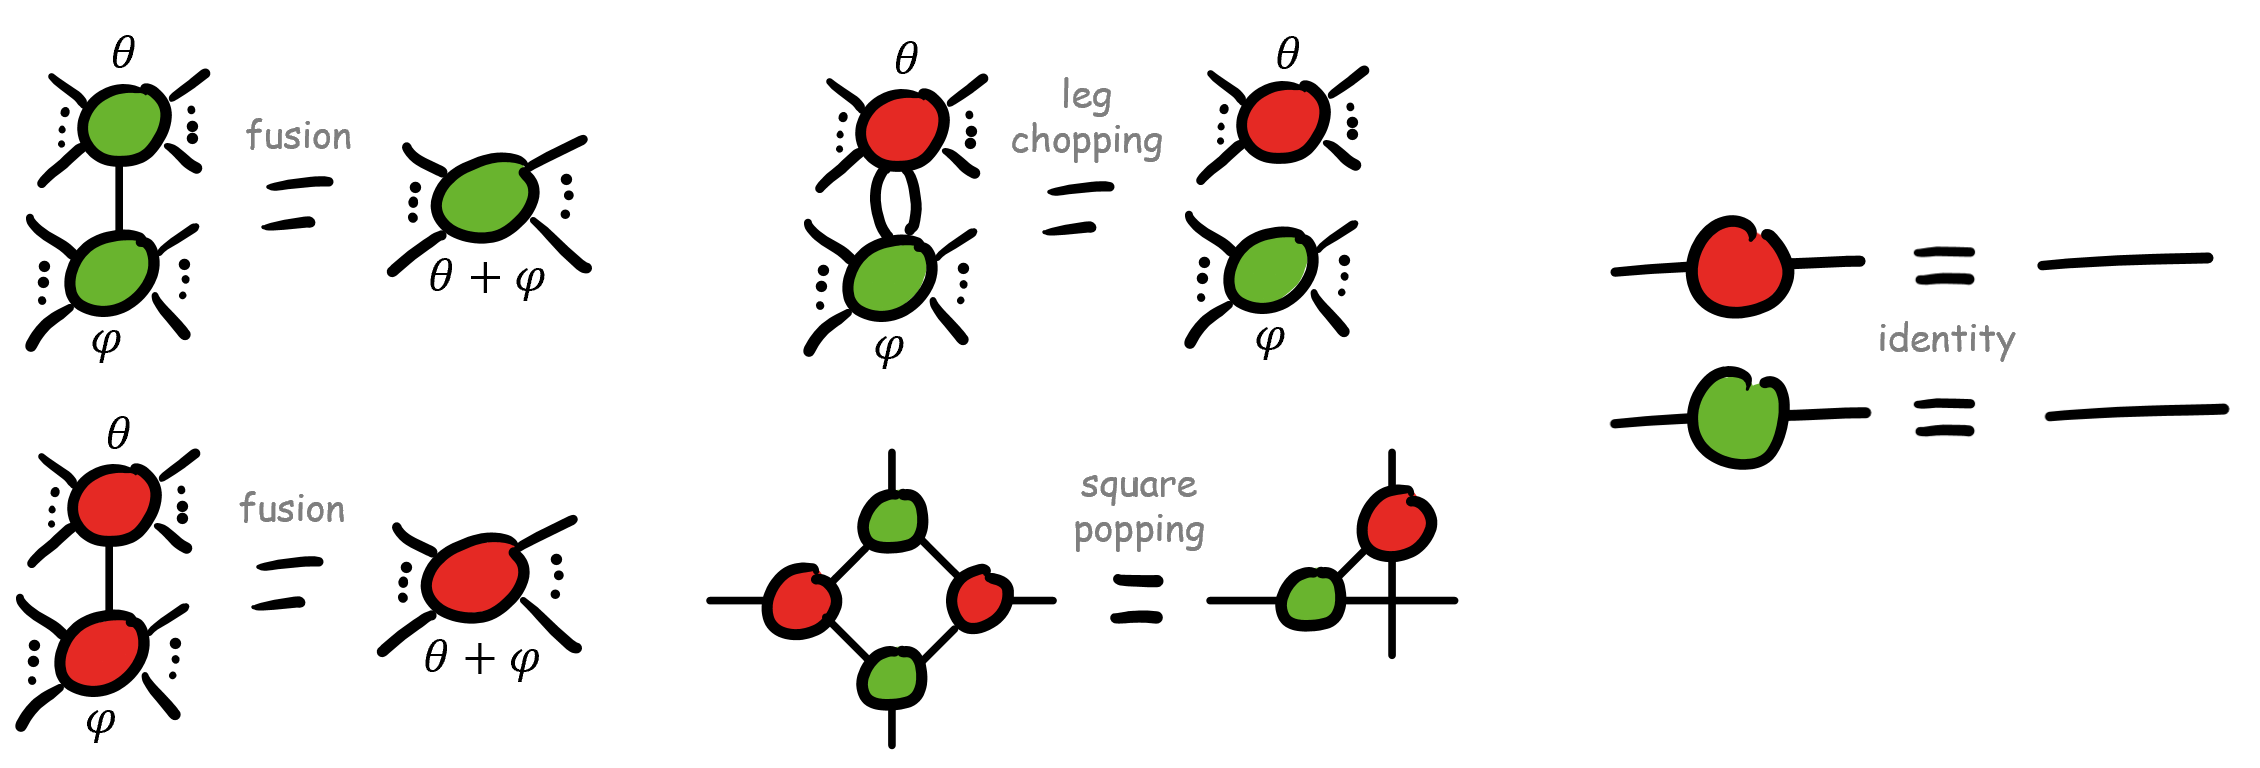
\includegraphics[width=0.8\textwidth]{Sections/pictures/zx-rules.png}
\caption{A selection of diagrammatic substitution rules for the ZX calculus, the visual language used by the Quantum Picturalism approach to Quantum Theory.}
\label{fig:zx-rules}
\end{figure*}

Figure \ref{fig:teleportation-learning} above exemplifies how quantum teleportation is introduced in a typical quantum information course.
It showcases two salient features of the traditional Hilbert space approach: (1) the heavy reliance on symbolic algebra---typically, Dirac's bra-ket notation---for the explicit description of quantum systems and calculations associated with their transformations; and (2) the need to employ a separate graphical notation---typically, quantum circuit notation---to explain the spatiotemporal layout of said quantum system and keep track of the operations acting upon them.
The shortcoming of the often-used combination of bra-ket notation and quantum circuit notation, is that the quantum circuit notation shows the operations of the protocol whereas the bra-ket computation shows the final result, but there is missing a representation of the intermediate steps bridging the two notations. In contrast, the QP proof makes clear the role of the Bell state and Bell measurement: The colors indicate that the CNOT gate, the $|0\rangle$ state, and the $|+\rangle$ state exhibit interaction of the Z (green) and X (red) observables, a fundamental observation that is not made evident by the quantum circuit, bra-ket, or matrix formalism. This corroborates previous observation that students in physics ``have difficulties with representations of quantum operators corresponding to observables especially when using Dirac notation''~\cite{Marshman2016difficultqoperators}. In a sense, the QP formalism makes it immediately clear that various components of quantum circuits are made ``of the same stuff'', and therefore interact in interesting ways (hence the title of the first ZX-calculus paper, `Interacting Quantum Observables'~\cite{coecke2011interacting}).

Below is the QP description of the quantum teleportation protocol, written in the diagrammatic language of the ZX-calculus.
Only two diagrammatic ingredients are needed: red and green circles---known as ``spiders''---annotated by angles and connected by lines.
The angles---known as ``phases''---indicate the extent to which qubits are rotated by various parts of the protocol, while the lines---known as ``wires''---indicate the exchange of quantum information (physical or virtual).
\begin{center}
    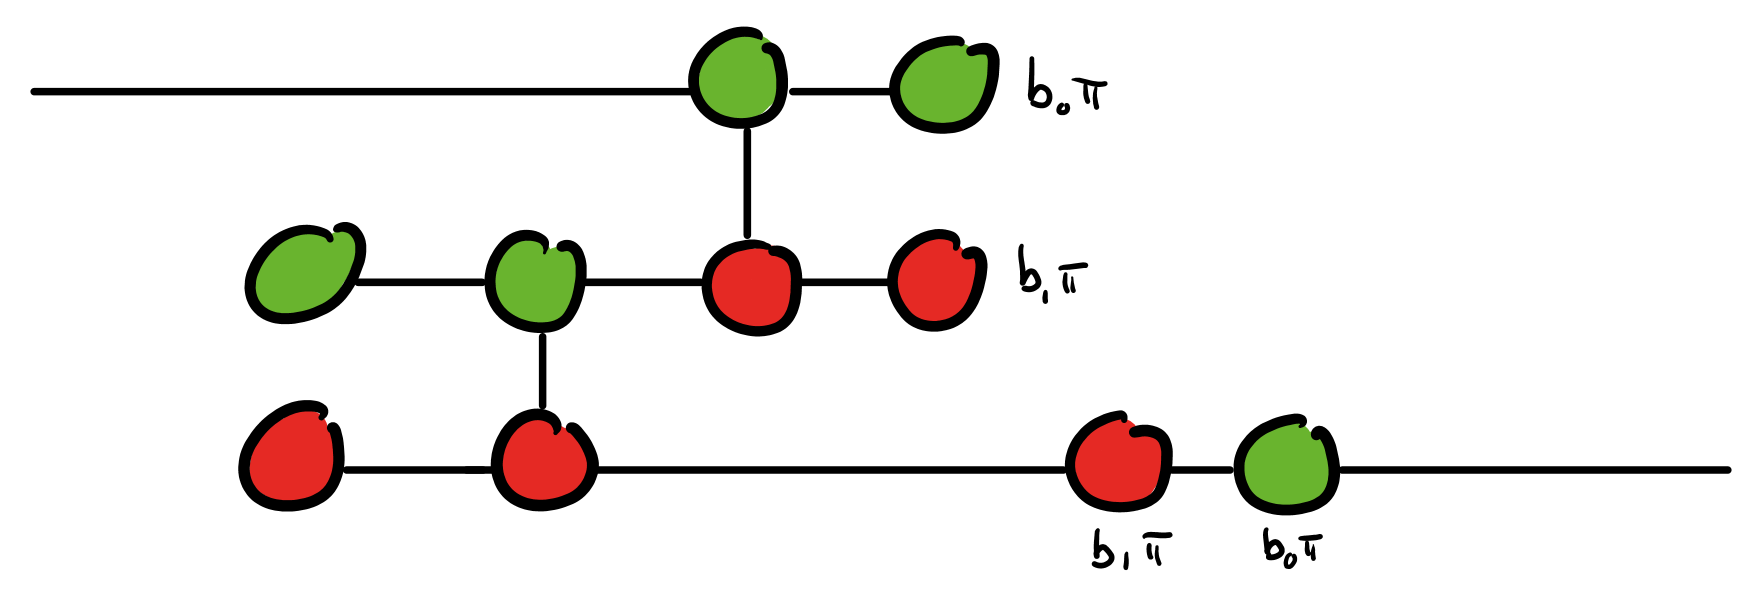
\includegraphics[width=0.4\textwidth]{Sections/pictures/teleportation-zx-raw.png}
\end{center}
Below is an annotated version of the same figure, indicating which parts of the ZX-diagram correspond to which parts of the traditional quantum circuit representation: the protocol takes a qubit as input (the wire on the left), results in a qubit as output (the wire on the right), and it involves two additional qubits, prepared in specified initial states (on the bottom left).
Two CNOT gates are applied to the three qubits, two of which are then measured (on the top right). A CNOT gate is a pair of a green spider and a red spider, connected by a vertical wire, with two wires on the left indicating the input qubits and two wires on the right indicating the output qubits.
The measurement outcomes, the bits $b_0$ and $b_1$, are then used to perform ``corrections'' on the remaining qubit in the form of two rotations (on the bottom right).
\begin{center}
    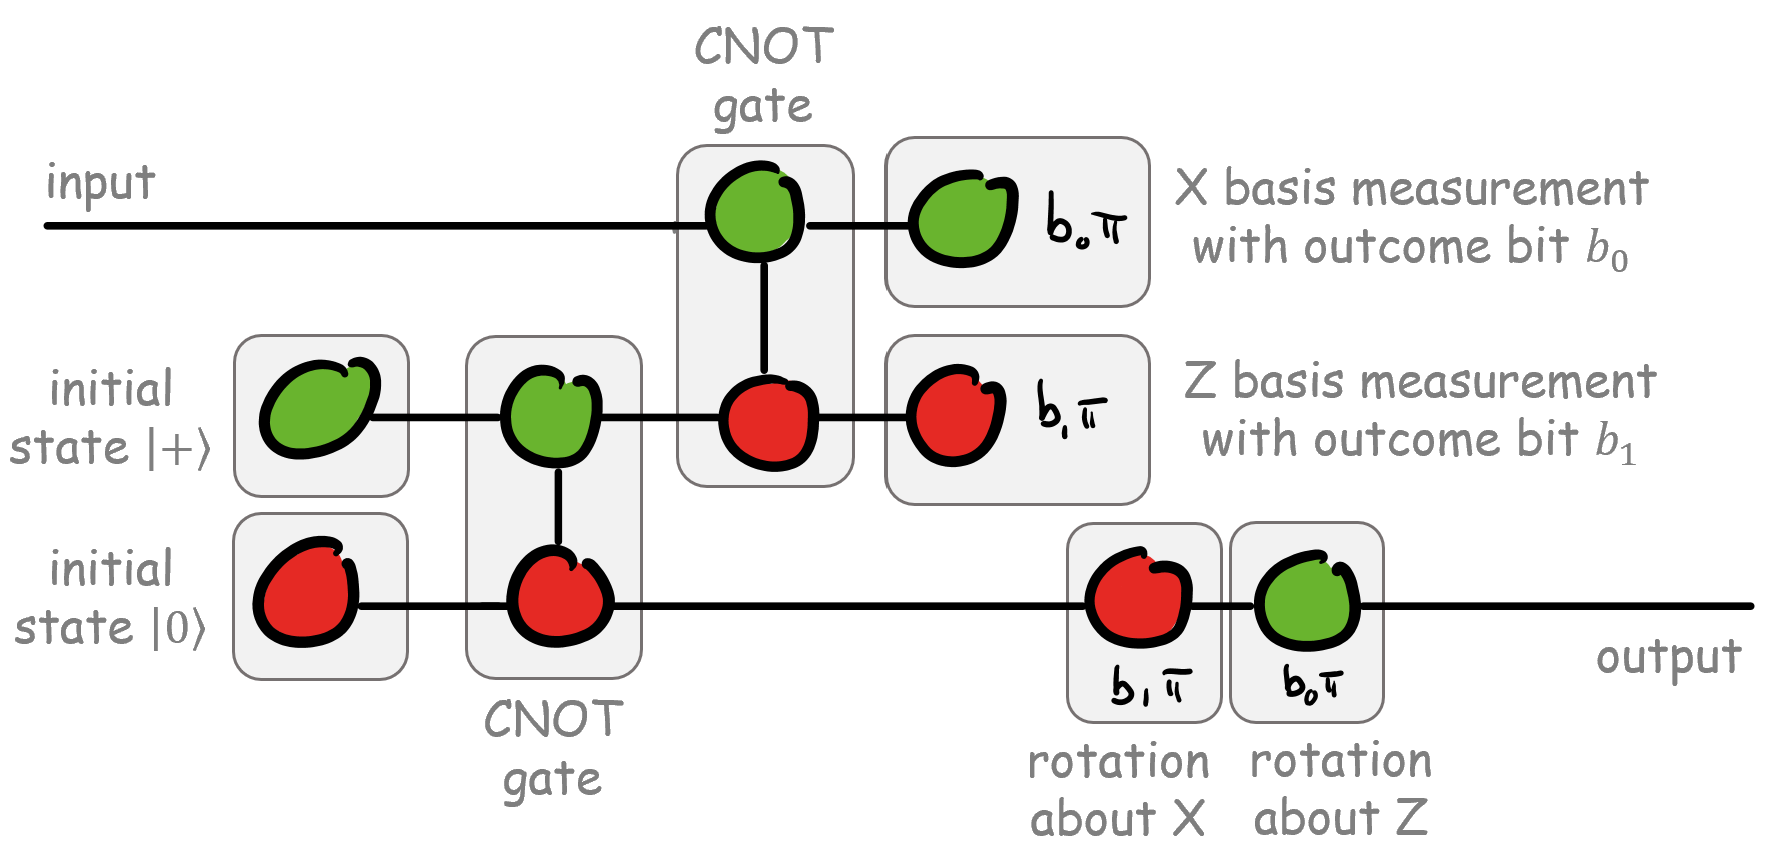
\includegraphics[width=0.45\textwidth]{Sections/pictures/teleportation-zx-annotated.png}
\end{center}
Without knowing much about the ZX-calculus, a comparison with Fig. \ref{fig:teleportation-learning} already highlights one of the critical features of QP: It reveals that parts which appear very different in the quantum circuit representation---initial states, CNOT gates and measurements---are composed of the same basic building blocks---red and green spiders---wired together in different patterns.

\begin{figure*}
\centering
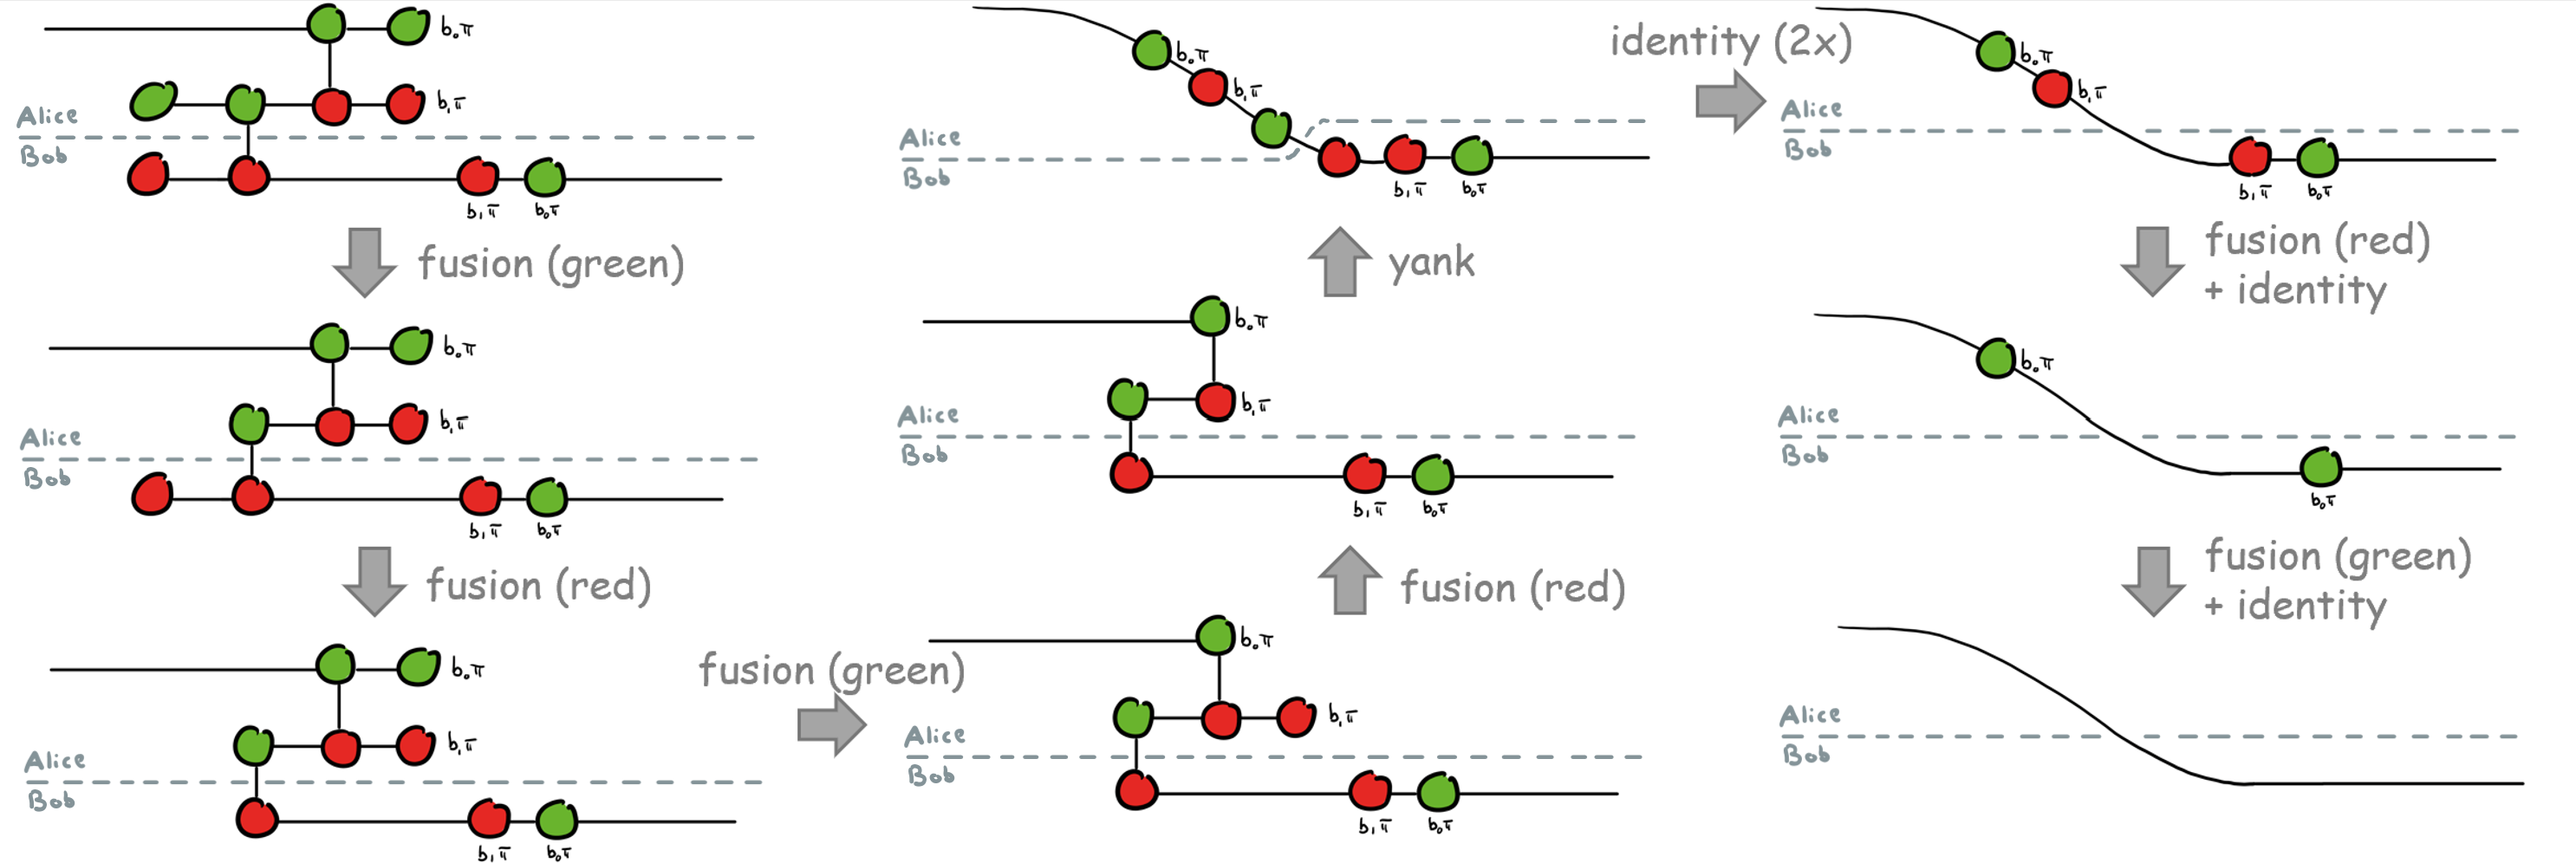
\includegraphics[width=\textwidth]{Sections/pictures/diagrammatic-reasoning-teleportation-steps-with-lines.png}
\caption{
Proof of correctness for the quantum teleportation protocol. This is the QP analogue of the Hilbert space calculations from Fig. \ref{fig:teleportation-learning} (p.\pageref{fig:teleportation-learning}). Each step of the proof is labeled with the diagrammatic rule of the ZX-calculus in Fig.~\ref{fig:zx-rules} used.
This elucidates the flow of quantum information. Here, it is clearer each operation in the quantum teleportation protocol contributes to sending quantum information from Alice to Bob.
The most important point of conceptual understanding is that the corrections Bob must make are precisely those which nullify the errors randomly generated by Alice's measurement; in other words, Alice's and Bob's Z and X spiders fuse to become zero phase spiders (phases of $2\pi = 0$ are unlabeled by convention), which can be removed by the identity rule.
Furthermore, the step of yanking the wires straight highlights a property of information flow in spacetime, namely that information is encoded by how spiders are connected, rather than by their placement on paper.
}
\label{fig:diagrammatic-reasoning-teleportation-steps}
\end{figure*}

The intent of the quantum teleportation protocol can be stated by the following diagrammatic equation, where the protocol (the diagram on the left) is stated to have the same effect (the equal sign) as moving the quantum state, without change, from its input to its output (the diagram on the right).
\begin{center}
    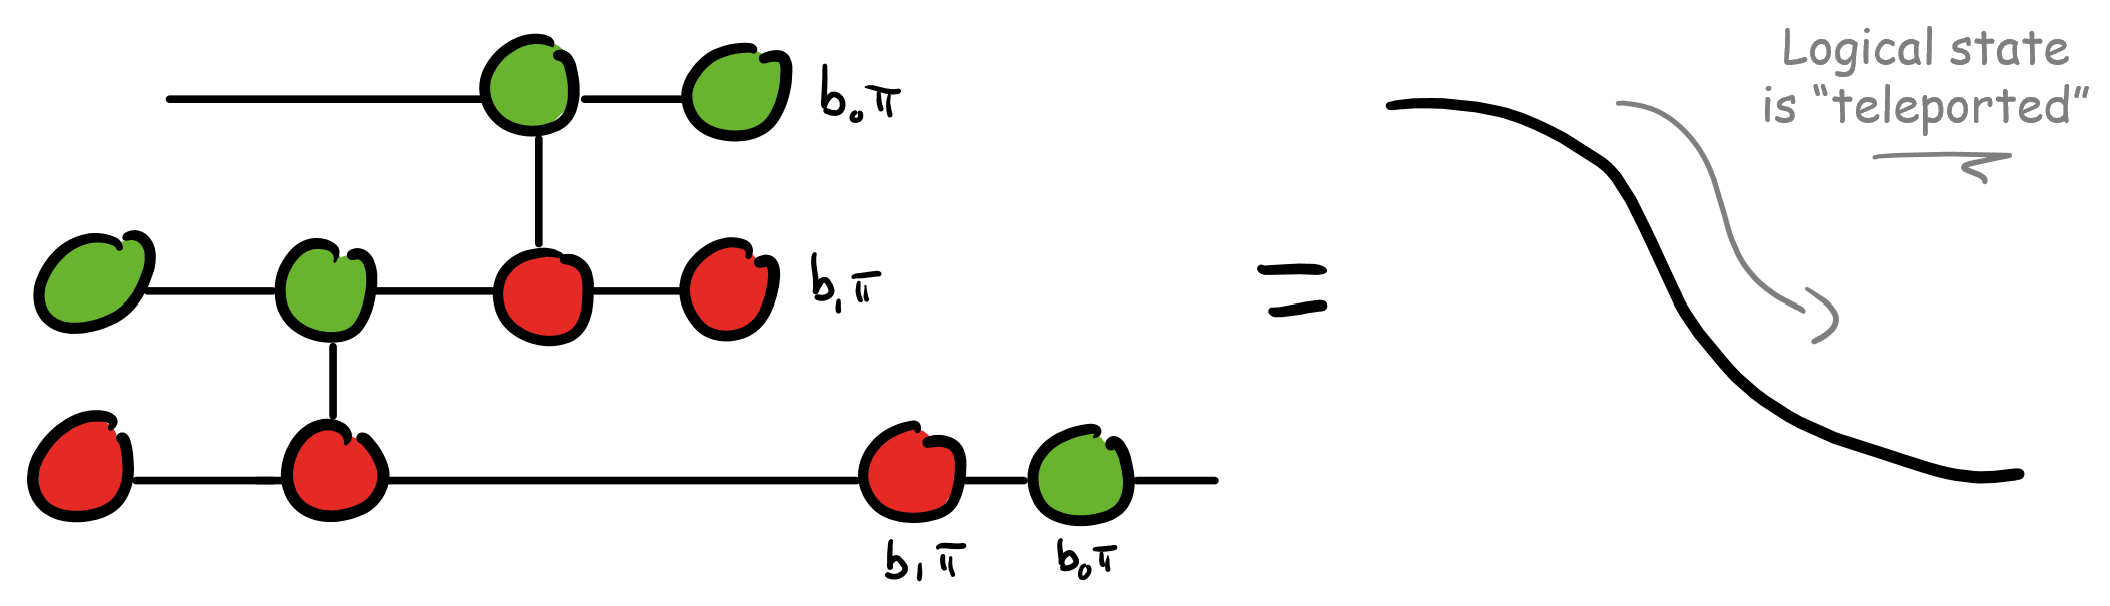
\includegraphics[width=0.45\textwidth]{Sections/pictures/teleportation-diag-reasoning.png}
\end{center}
In the QP approach, the same diagram that describes the protocol simultaneously provides the medium upon which any associated calculations can be performed.
This contrasts with the traditional Hilbert space approach, where different languages are used for calculation (bra-ket notation) and description (quantum circuit notation).
Calculations in the QP framework proceed by applying ``substitution rules'', graphical modifications of diagrams that maintain their meaning, i.e. that result in different diagrams with the same effect (symbolised by the equal sign).
Figure \ref{fig:zx-rules} (p.\pageref{fig:zx-rules}) presents some of the substitution rules for the ZX-calculus used by the examples in this paper. With the addition of only a few more other rules to the ones shown in Fig. \ref{fig:zx-rules}, the set of substitution rules is complete, i.e. suffices to make the ZX-calculus as expressive as the Hilbert space formalism for qubits~\cite{hadzihasanovic2018two} and more generally, for arbitrary finite dimension~\cite{poor2023completeness}.

As a warm-up exercise in diagrammatic substitution, below is the proof that two CNOT gates in sequence cancel each other out, leaving the two qubits---the two wires running left to right---unchanged.
\begin{center}
    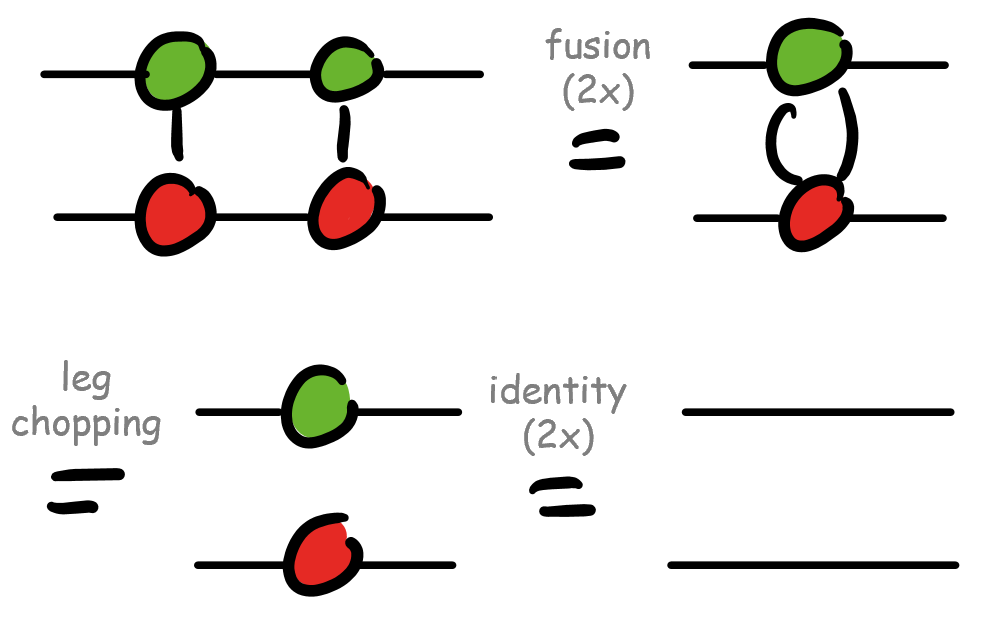
\includegraphics[width=0.3\textwidth]{Sections/pictures/double-cx-two-lines.png}
\end{center}
The proof consists of two steps.
As the first step, we apply the ``fusion'' rule twice (cf. Fig. \ref{fig:zx-rules}, left): once to fuse the two green spiders, once to fuse the two red spiders.
As the second step, we apply the ``leg chopping'' rule (cf. Fig. \ref{fig:zx-rules}, middle top), to remove the pair of legs between the red and green spiders.
The results are two undecorated wires, carrying the two qubits from input to output unaltered.

% As a second warm-up exercise, below is the proof that three alternating CNOT gates have the same effect as swapping two qubits.
% This is an important practical observation in quantum computing, use to compile quantum circuits in architectures---such as superconducting quantum computers---where CNOT gates can only be performed between a small number of qubit pairs.
% \begin{center}
%     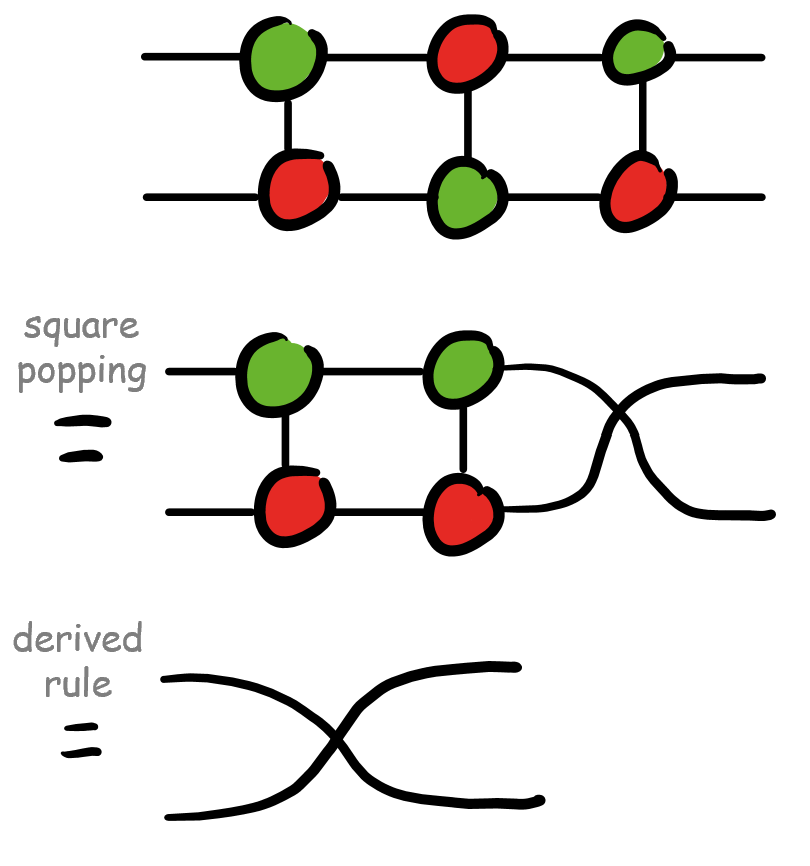
\includegraphics[width=0.25\textwidth]{Sections/pictures/triple-cx-three-lines.png}
% \end{center}
% The proof consists of two steps.
% As the first step, we apply the ``square popping'' rule (cf. Fig. \ref{fig:zx-rules}, middle bottom) to the rightmost two CNOTs, replacing them with a CNOT and a qubit swap.
% As the second step, we apply the equation from the previous exercise as a ``derived rule'', removing the two CNOTs and leaving the desired swap.

Now familiar with the diagrammatic substitution, we can focus on Figure \ref{fig:diagrammatic-reasoning-teleportation-steps} above, presenting the full proof of correctness for the quantum teleportation protocol.

The natively visual character of QP makes it easy to augment diagrams with other kinds of visual information, synergistically enhancing the communication power of all media involved.
For example, below is an explanation of how the fusion rule (cf. Fig. \ref{fig:zx-rules}, left) implements the action of rotation gates on quantum states.
\begin{center}
    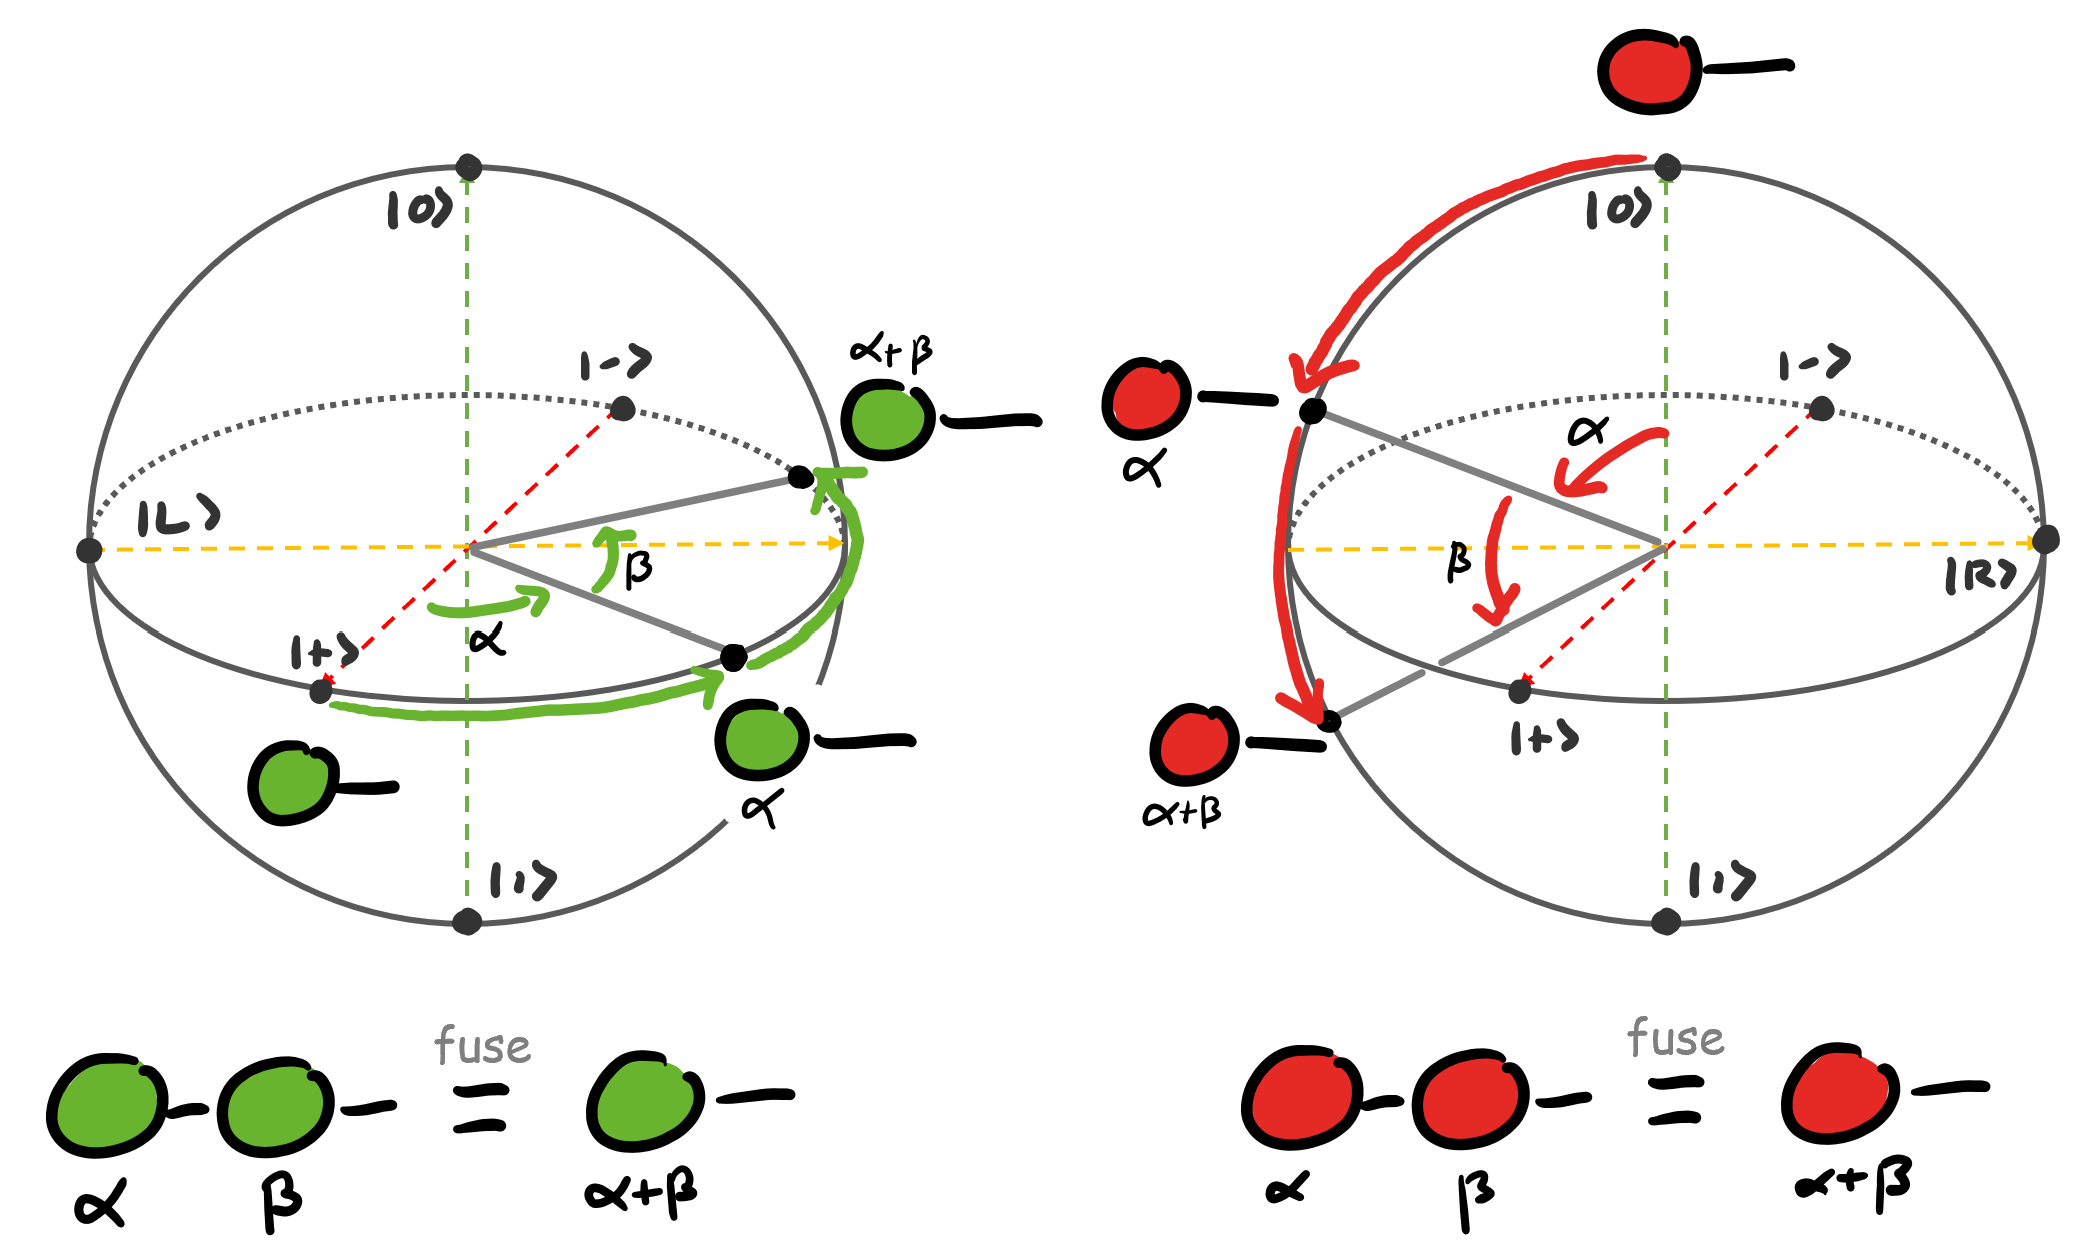
\includegraphics[width=0.5\textwidth]{Sections/pictures/spider-states.png}
\end{center}
The Bloch spheres endow the spiders with additional geometric meaning, locating them on the equator and prime meridian based on their phase.
The fusion rule, on the other hand, enhances the Bloch sphere presentation by adding a dynamical, computational description of the rotation action.

Diagrams are also easily augmented by non-technical conceptual art to convey meaning that exceeds the boundaries of mathematical and physical rigour.
For example, below is a diagrammatic representation of the Bell test, where an entangled state is measured simultaneously by two parties at a large distance apart.
\begin{center}
    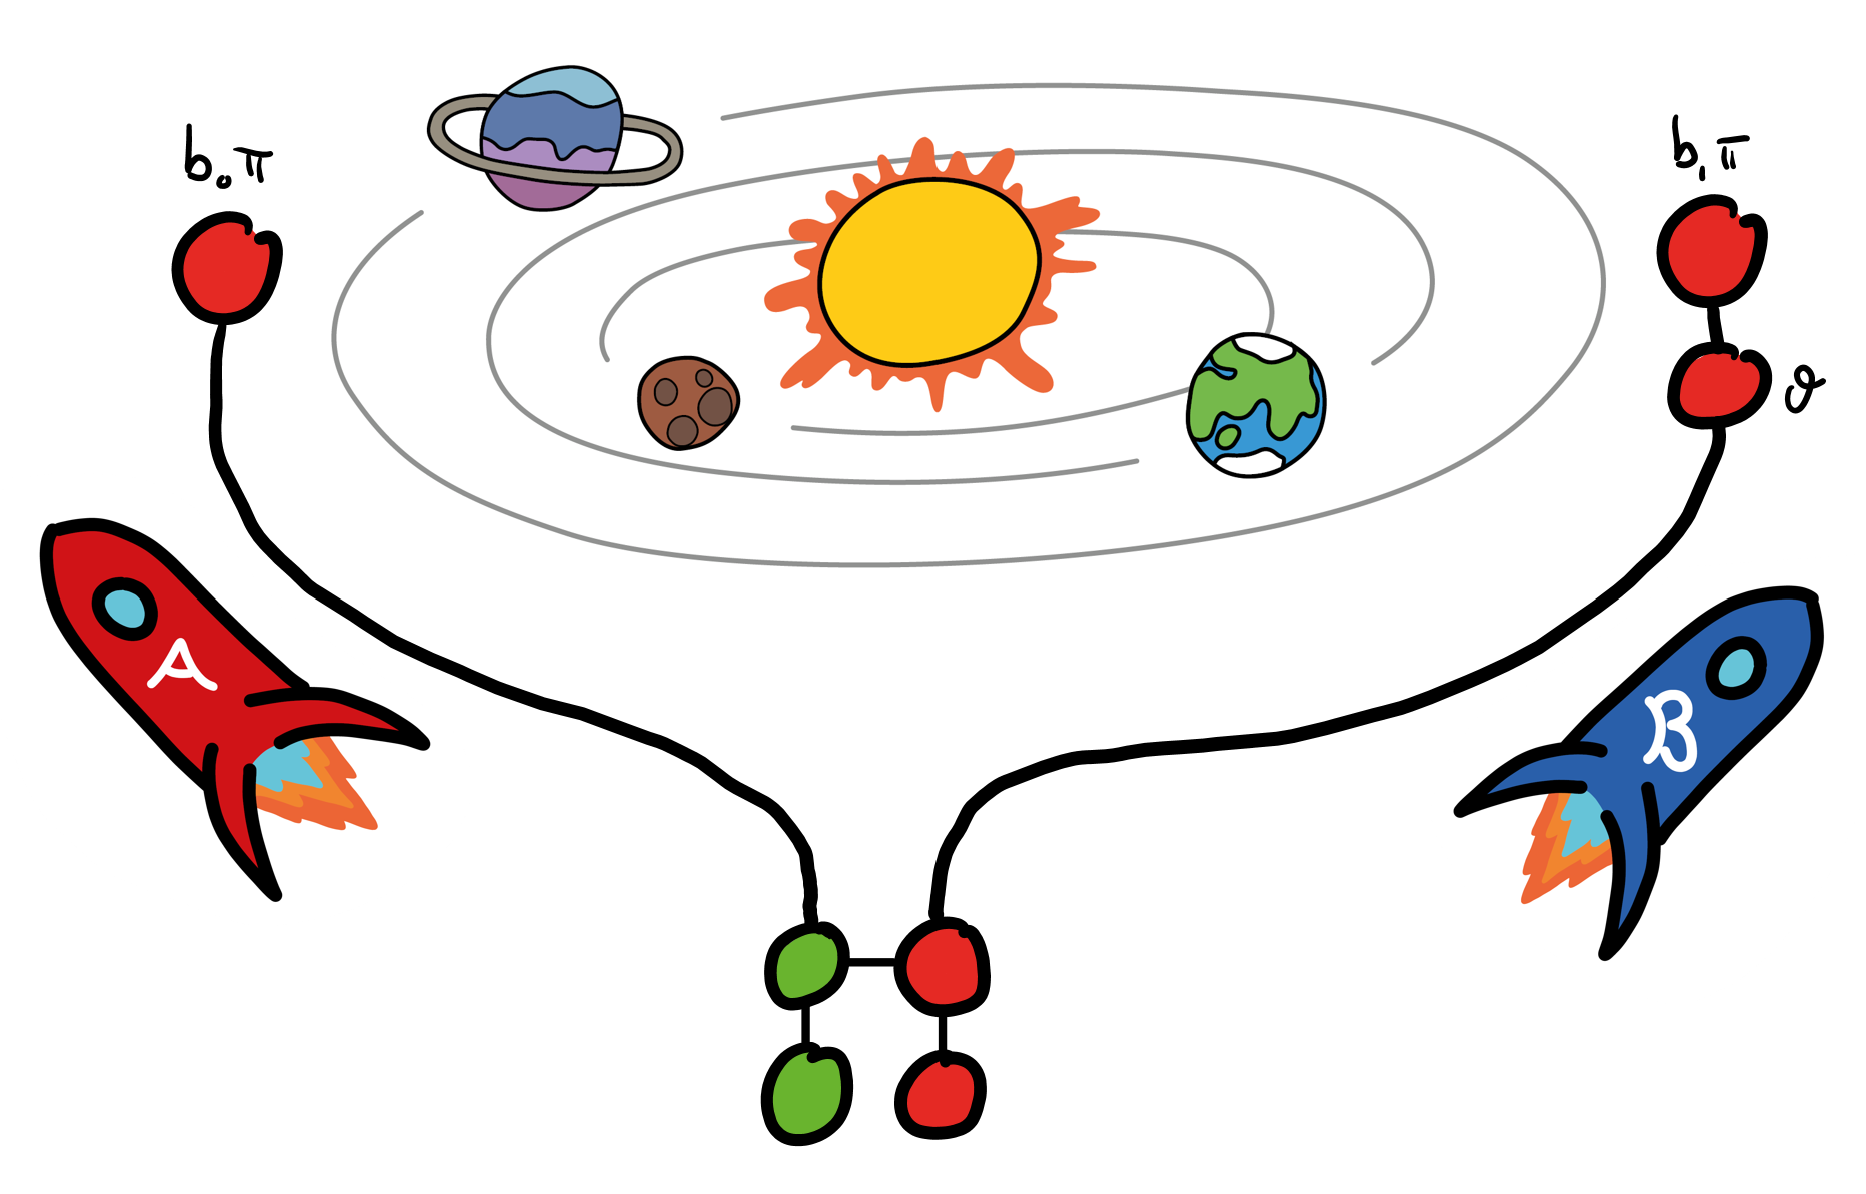
\includegraphics[width=0.4\textwidth]{Sections/pictures/diagrams-mixed-media.png}
\end{center}
The diagram is enriched by a number of artefacts and considerations.
Firstly, the diagram is drawn bottom-to-top\footnote{As opposed to the left-to-right convention, which we have previously adopted to represent the quantum teleportation protocol, matching the directional convention of quantum circuit notation.} to match worldline diagrams from general relativity.
Secondly, drawings of rockets and a solar system are used to indicate that, after becoming entangled, the two qubits are moved very far from each other.
Finally, the two measurements are horizontally aligned to indicate the (approximate) simultaneity of the operations performed by the two parties at a distance.

Finally, the diagrammatic representation itself can reveal hidden spatial structures within quantum algorithms, which may help explain how and why such algorithms work.
For example, below is a diagrammatic representation of the Quantum Approximate Optimisation Algorithm (QAOA), applied to solve the max-cut problem\footnote{An important combinatorial optimisation problem on networks. The max-cut problem is ``NP-complete'', i.e. solutions to this problem translate into solutions for a large class of problems of enormous real-world significance.} on a small network (6 nodes, corresponding to 6 qubits).
The traditional presentation of this algorithm (left below) uses initial states, CNOT gates, Z rotations and measurements, much as the quantum teleportation algorithm previously discussed.
By exploiting the visual flexibility of the QP approach, we repeatedly apply the fusion and square-popping rules (cf. Fig. \ref{fig:zx-rules}) and re-arrange the spider layout until the simplified diagram (right below) is obtained.
\begin{center}
    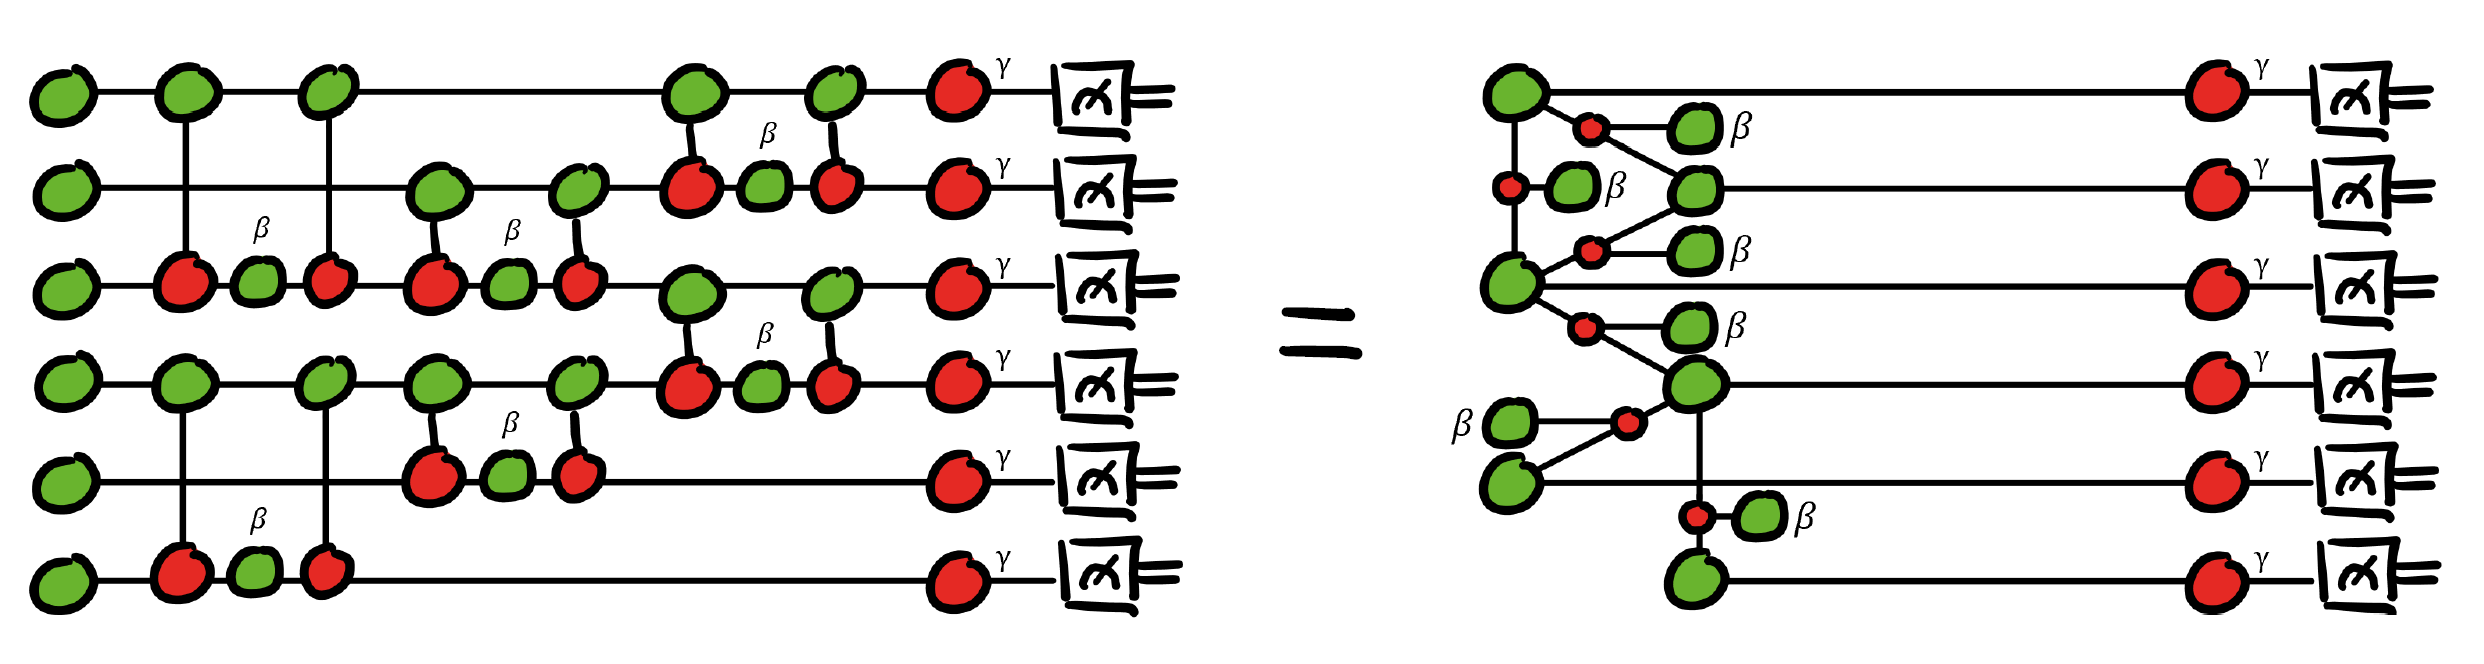
\includegraphics[width=0.48\textwidth]{Sections/pictures/diagrammatic-reasoning-qaoa-eq.png}
\end{center}
The structure of the network (6 nodes connected by 6 edges, drawn in blue, left below) is revealed within the simplified and re-arranged diagram (spiders and wires highlighted blue, right below), exposing the mechanism that ultimately powers QAOA: the ability to entangle quantum systems in a way which matches the constraint pattern of the chosen optimisation problem.
The algorithm parameters---the $\beta$ and $\gamma$ angles below---allow the quality and degree of entanglement to be tuned, exploring the space of solutions in directions determined by the entanglement pattern.
\begin{center}
    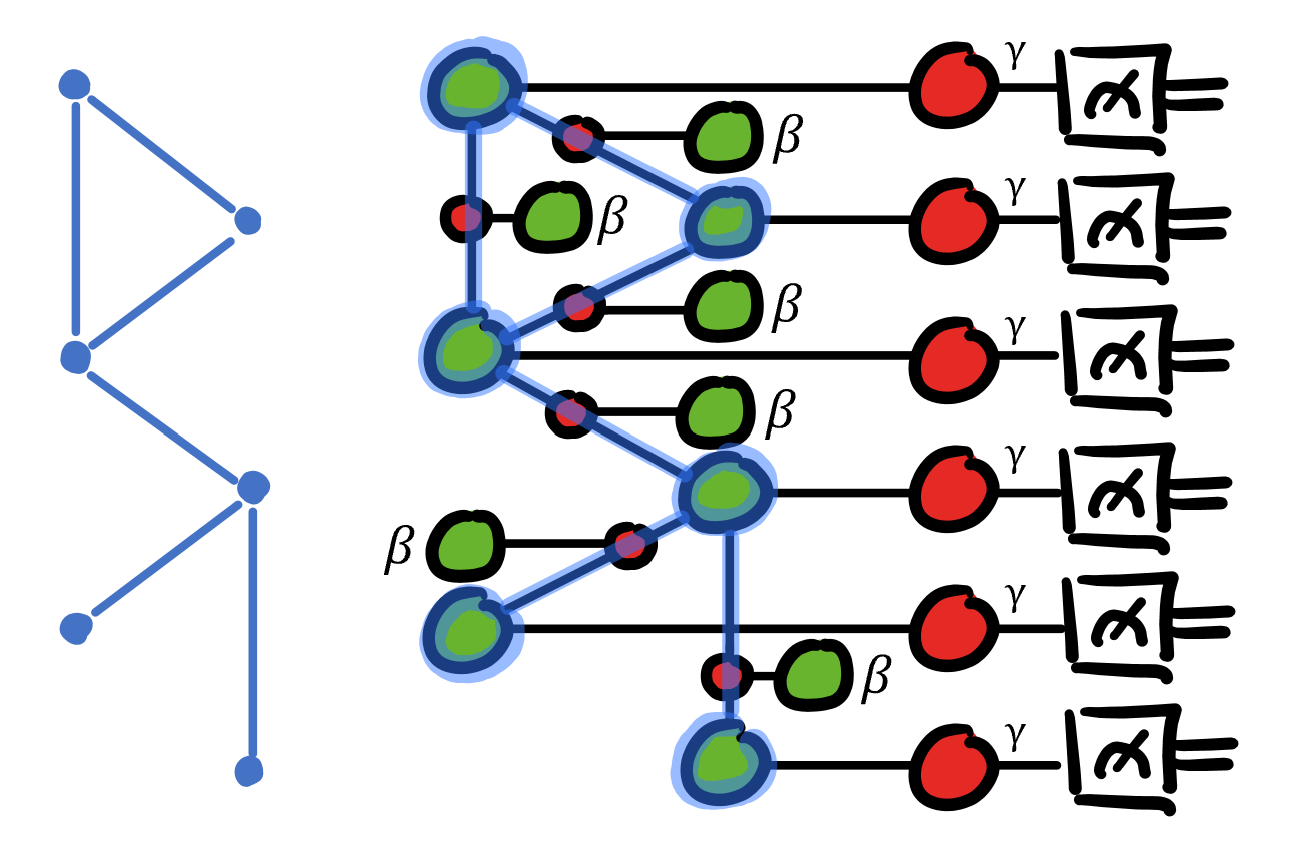
\includegraphics[width=0.34\textwidth]{Sections/pictures/qaoa-circ.png}
\end{center}


% In analogy to the history of classical computer science, the Hilbert space formalism is to low-level assembly code what QP is to high-level programming languages. The Hilbert space formalism may have well been enough to get us through the early days of quantum computer science, but the exponential increase in complexity will soon necessitate higher-level methods, to bring forward applications that would be unimaginable with low-level conceptual tools alone.

\section{Experiment and evaluation}
\label{sec:xpmt}

This project was designed to collect evidence through an intervention trial to test whether (1) the diagrammatic formalism provides the most effective method to present quantum information theory (QIT) content, and (2) this formalism can significantly enhance young learners’ problem-solving ability after their training.


\subsection{Design and sampling}

This intervention trial is scheduled to be implemented between the 5th of June and the 11th of August, 2023.
It is designed to be delivered online through weekly one-hour sessions, each following a half an hour of self-study, spanning 10 weeks.
Through this trial, evidence has been 
 collected using a post-test design to evaluate the effectiveness of the QP approach.
A purposive sampling approach was employed to recruit 75 volunteer high-school students aged 16 to 19. The sample size was determined based on the number of available tutors. 

The project flyer was distributed to approximately 26 high schools across the UK and promoted on various social media platforms. Despite reaching out to a limited number of schools and teachers due to time constraints, we have received a more significant number of applications than anticipated $(N_0=734)$ within three weeks.
To ensure the quality of training, we  conducted an initial filtering process to exclude non-high-schoolers, respondents outside the target age range, and non-UK students as mandated by the obtained ethical approval.
We then asked for a study commitment of two hours weekly for 10 weeks, and sampled a random subset of positive respondents to reflect a balance of diversity criteria, re-sampling random subsets of respondents until all criteria were met within predetermined accuracy.
A total of 75 candidates were selected, with the goal of around 50 of them completing the course, taking into account potential attrition.

Participants have been provided with the experiment handbook that effectively communicates the objectives and requirements of the study; outlines the schedule; describes the evaluation methods to be used after the training; provides procedures for the tutorials; covers data protection and privacy policies; provides relevant contact details; and includes a handout which summarises the post-training procedures.
They have also been provided with a slimmed-down version of the QP book by Coecke and Gogioso~\cite{coecke2022quantum} to act as their tutorial book.
A similar and more substantive textbook by Coecke and Kissinger~\cite{CKbook} is actively  in use in various university-level courses, most notably at the University of Oxford.

All participants have been granted access, via a secure link, to weekly online recorded lectures (episodes) specifically designed to teach QP (a brief outline of the content is provided in Appendix A). They were also expected to engage in half-hour self-study sessions before the scheduled tutorials.
This was to help mitigate the effect of teacher and tutor variation on training outcomes, as each participant needed to have access to the same lectures during training via the project portal.

Participants have been provided with a link to book tutorials at their convenience. Each week's practice tutorials have been conducted by one of eight tutors, with a class size of 15 students maximum per tutorial.
 
To reduce the effect of tutor variation, the carousel technique was implemented: tutors rotated weekly, with a dedicated tutor being responsible for the week's material, enabling them to interact with each group at least once during the training period.
Consultation sessions with team members and tutors took place during the 1st, 3rd and 6th weeks to enable tutors to share their experiences and discuss the implementation of necessary measures.

Tutors underwent a Disclosure and Barring Service (DBS) check following UK regulations and completed a one-hour training session ahead of the trial. The training covered the study's objectives, effective interaction with students, conflict management, strategies for handling students with varying abilities, guidelines for taking observational notes for later qualitative data analyses, and techniques for encouraging students to progress towards the next steps.
It was made clear that the tutorials would primarily focus on practical exercises within interactive sessions.

Our tutors are highly qualified doctoral students, lecturers from the University of Oxford, and researchers from Quantinuum, all with substantial teaching experience.
Tutors were explicitly instructed to devise their own plans for implementing additional examples to reinforce the video lectures. These plans were supported by the Principal Investigators (PIs), who assisted in various aspects, including providing additional examples for each tutorial week. Their support ensured the curriculum remained up-to-date and incorporated research expertise and industry knowledge. 

\subsection{Data collection procedures}

Participants’ performance changes in learning outcomes (outlined in Appendix A) has been monitored via tutors' notes every week leading up to the post-tests. The weekly monitoring helped determine whether individuals exhibited observable improvement as a result of the training. For this, we utilised both directly related measures of performance and qualitative assessments of achievements. 
In addition to tutor notes, the exam and attitude questionnaires evaluated participants’ performance, providing comprehensive data to assess their progress and attitudes toward the training.  

\subsection {Assessment and evaluation}

The exam questionnaire used in this study is identical to the one previously implemented by the PIs in the quantum physics course for undergraduate students at the University of Oxford.
The questions were specified by the PIs for this project and subsequently reviewed by two project members to evaluate their applicability, appropriateness, language, presentation style, variability, and representativeness.

Questions were chosen to test the level of proficiency across target skills, ranging from calculation by diagrammatic manipulation to conceptual understanding of quantum information scenarios represented by the diagrams.

The selection process for each question involved careful consideration of various factors, including: 
\begin{itemize}
    \item objectives and aim of the study,
    \item desired outcomes,
    \item relevant literature,
    \item previous implementations with undergraduate students,
    \item the expertise of the PIs, and input from the research team, 
    \item a review process to assess the questions' clarity, relevance, and appropriateness for the study population. 
\end{itemize}

Upon completing the 8th week of training, participants were given a two-week period to complete and submit their answers to the exam questions.
The submitted work underwent a rigorous marking process managed by two experienced PIs, Coecke and Kissinger, who have been marking similar work for over a decade. They independently assessed students' work by following the provided criteria in Appendix B. This ensured fairness and accuracy, where each examiner independently assessed the submission without knowing the other's decision. In cases where a significant discrepancy of more than 9\% in the assigned grades occurs, another PI, Gogioso, was involved to review and facilitate further discussion until a consensus is reached.
This ensures consistency and transparency in the marking process, aims to provide participants with clear evaluation criteria and constructive feedback alongside their marks, and maintains consistency in the final grades.  

Participants' attitudes were assessed before the trial, focusing on three aspects: (1) their commitment, (2) interest in pursuing a STEM career, and (3) providing at least one specific reason for their interest in participating.
The post-intervention attitude assessment gathered feedback on the overall setup, satisfaction with the tutorials, any changes in their career plans, and their post-training/future expectations. Additionally, an optional question regarding their grades in STEM subjects was included to aid in analysing correlations between exam scores and attitude questions.
The attitude assessments generated qualitative data, which will be analyzed using qualitative analysis techniques in a follow-up study.

\subsection{Measured variables}

The outcome variables for the assessment, derived from the two questionnaires above (exam and attitude), focus on the number of problems students successfully solve using QP. 

The marking scheme prioritized comprehension rather than solely assessing the overall accuracy of answers. The evaluation process was guided by the following rubric, which is designed to align with the objectives, learning outcomes, and analysis scheme outlined in the breakdown marking criteria provided in Appendix A:

\begin{itemize}
\item Methodology: Assessing general problem-solving skills, including problem analysis, the ability to break down complex problems into smaller components, and logically organize the steps required to find a solution.
\item Correctness: Evaluating the accuracy of solutions and the validity of the reasoning provided in the answers.
\item Conciseness: Assessing the ability to present solutions concisely, considering factors such as the number of steps required to reach a solution.
\item Originality/Creativity: Considering the creativity and originality of the strategies employed by students in solving problems.
\item Evidence of understanding: Evaluating the correct application of relevant concepts and strategies taught during the course, such as the appropriate use of diagrammatic rewriting rules, and demonstrating a deep understanding of the physical meaning behind concepts like diagrammatic quantum teleportation.
\item Structuring, communication, presentation: Assessing the ability to organize, write, and draw solutions in a clear and unambiguous manner. This includes aspects such as the proper use of colors, distinguishing between ``quantum'' and ``ordinary'' diagrams, and using terminology consistent with the content presented in the tutorials (e.g., ``square-popping'', ``leg-chopping'', etc.).
\end{itemize}

Self-reports were also taken into account during the post-test period, in conjunction with the weekly observational data collected by tutors. Tutors received a feedback form they completed after each week's tutorial. This was to facilitate the assessment of each student's progress throughout the training and enable meaningful comparisons.

Further demographic factors, such as age, parental education, English language proficiency, and school type, were analysed as independent variables within the socio-economic and cultural impact on performance.

\subsection{Data exclusion rule}

Participants have been informed that they can withdraw from the study at any point.
Attendance during the training period was monitored, but only data from participants who attended tutorials and completed post-testing were included in the analysis.
As per the attendance rules agreed during the recruitment stage, participants had to register for one of five tutorial time options each week.
%Participants who were absent for more than one week of the online tutorials were excluded from the study.

To prevent the spillage  effect, participant interactions were discouraged during and after the training until they had submitted their exam answers. They were requested to keep their personal information private from each other to uphold the integrity of their training and ensure the validity of the analyses. With these precautions in place, no  unsupervised interaction or violation of research protocols between participants was observed  that would require us to exclude their data from the analyses, ensuring the study's validity. 

\subsection{Data Transformations}

For privacy reasons, raw subject data stored in a single/secure location accessible only to the project PI, Kissinger.
Students were then assigned a unique code to enable anonymised data to be shared and analysed independently by research team members. 
The researchers worked together throughout the data collection process, following the protocols for test administration. 
As a follow-up, frequency tables generated for each variable using SPSS / R to check that there are no out-of-range values and that any missing data points have been appropriately coded.
This strategy of creating single intermediate records, collating all raw data relating to each participant, has proved to be an essential facilitator of data checking and cleaning before entry for analysis, and tabulated data can be set up to allow for semi-automated entry once this process has been completed. 
Once data collection was ongoing, the researchers double-checked the processes involved, including coding and storing the raw data from the testing.
The coding schemes were modified where necessary.

\subsection{Analysis}

The impact of training was measured via post-tests.
Effects were assessed using analysis of variance. Differences in performance between the age groups were assessed using hierarchical regressions, path analyses, and multilevel modelling, also aiming to examine the influence of socioeconomic and demographic factors. 
Furthermore, underlying attitudinal factors examined using exploratory factor analysis. 



\section{Discussion}
\label{sec:discuss}

Recently, there has been a resurgence of interest in exploring the quantum foundations of the universe, accompanied by a notable acceleration in the advancement of practical quantum technologies---a phenomenon sometimes known as the ``second quantum revolution''~\cite{dowling2003quantum}. However, a sound understanding of quantum theory has yet to penetrate mainstream awareness, education, and the professional training pipeline.

To make quantum knowledge accessible to a broader audience, we must  present complex scientific phenomena in a way that is more readily suitable for learning. This requirement necessitates a deviation from traditional approaches, which rely too heavily on complex symbolic reasoning and highly technical language. Additionally, our presentation should be practically applicable, as opposed to approaches which rely on inaccurate metaphors to convey a simplified, intuitive understanding of a complex subject matter. The experiment detailed in this paper proposes QP \cite{ContPhys} as a viable candidate for such a presentation, in the form of a visual paradigm already adopted in the wild for lecturing \cite{CKbook, coecke2023basic}, reasoning \cite{van2020zx}, and research \cite{de2020fast, de2019techniques, kissinger2019reducing, de2020zx, kissinger2022phase, khesinGraphicalQuantumCliffordencoder2023}.

This experiment is unique in three aspects.
Firstly, it offers state-of-the-art educational material, tailored to empower participants to perform quantum calculations using the diagrammatic formalism. Rather than merely advocating a `shut-up-and-calculate' approach, the curriculum presents a new conceptual foundation for learning physics and science, both quantum and beyond, with primary focus on a holistic understanding of the relationship between events and processes.
This unique perspective not only simplifies the formalism, but also supercharges the users' reasoning skills about quantum systems and their otherwise puzzling behaviours.

Secondly, the experiment aims to assess whether QP can democratise access to a crucial segment of university-level education by extending its reach to high school students. For almost a decade, QP has been taught to a small selection of students at elite universities, most notably the University of Oxford. As part of our experiment, a more diverse group of students---in terms of academic background, gender, socioeconomic status, and prior mathematical knowledge---will reap the benefit of QP for the first time.

Thirdly, the experiment explores whether learning quantum theory falls within the zone of proximal development of high school students, i.e. whether adequate guidance and support can enhance their understanding of such a subject matter.
A successful experiment would settle the question in the positive, while an unsuccessful outcome leaves the possibility that the experimental setup did not provide sufficient guidance to fully bridge the gap between the high-school syllabus and the more specialised requirements of quantum disciplines.

More evidence will be needed to test against diverse control groups, and to explore the effects of QP on larger samples of the high-school student population.
The facilitating effect of QP on the acquisition of quantum technology skills will also require further evaluation, investigating how it assists novices in accurately organising their mental representations while minimising the cognitive resources needed to achieve proficiency in real-world tasks.

The insights gained from this and future work will undoubtedly pave the way for the development of more inclusive and innovative educational endeavors. These efforts will play a significant role in bridging the gap between high school and university level learning, particularly for those aspiring to pursue a STEM career. It will help them establish crucial conceptual and abstract frameworks earlier, significantly contributing to their academic growth and understanding. 

Finally, the findings have the potential to inspire further research and advancement in quantum science pedagogy, contributing to the ongoing evolution of educational methodologies and practices specific to quantum technology and beyond. 



\section*{Appendecies}

\section{Content and learning outcomes}

Below is the detailed week-by-week breakdown of course content and learning outcomes:

\begin{itemize}
\item In week 1, the episode ``Quantum in Pictures: Wires and Boxes'' introduces diagrams composed of wires and boxes to describe processes and perform mathematical operations. The episode also introduces the concepts of space and time in diagrams and the physics they represent.
\item In week 2, the episode ``Quantum Teleportation'' introduces the concept of the quantum lottery and the idea that wires and boxes can be used to carry out advanced mathematical reasoning. It then discusses quantum teleportation, a fundamental building block of quantum communication and quantum computing.
\item In week 3, the episode ``A World of Spiders'' introduces ``spiders'', a special kind of box with basic rules to work with them. Spiders---discussed in Section II on Quantum Picturalism---provide the fundamental building blocks for quantum computing.
\item In week 4, the episode ``Quantum Computing'' introduces quantum computing using spiders: logical operations (such as copying and adding), quantum gates (such as rotations, CNOT gates and Hadamard gates) and measurements.
It covers the use of diagrammatic substitution rules for circuit simplification and other relevant calculations.
% Classical computers use bits, and quantum computers use qubits. The episode covers the representation of bits and qubits using spiders "decorated" with phases. The episode also covers logical operations on those (qu)bits, like copying, adding, and the CNOT gate using spiders. For example, the CNOT gate is composed of a green spider and a red spider connected to each other---discussed in Section II on Quantum Picturalism. Participants also learn how the Hadamard gates (colour-changing boxes), introduced in the previous episode, affect a circuit of spiders. Learning how applying rules on spiders helps realise computations (\emph{i.e.} given quantum states at the beginning of a circuit, what are the quantum states at the end of the circuit, and the output of the computation) and simplify circuits, valuable to experimentalists with limited resources.
\item In week 5, the episode ``Quantum Teleportation with Spiders'' explores quantum teleportation further. It then introduces measurement-based quantum computing (MBQC), a fault-tolerant flavour of quantum computing which uses ideas from quantum teleportation to shift computation from gates to measurements. MBQC was also one of the motivating examples in developing the ZX-calculus.
\item In week 6, the episode ``Keeping Einstein Happy'' introduces notions of relativistic causality within the diagrammatic framework in the form of Sure-boxes and Maybe-boxes. 
\item In week 7, the episode ``Quantum vs Ordinary Particles'' introduces the concept of double wires to distinguish the quantum world from the classical world. Mathematically, doubling the wire gives new kinds of numbers (real probabilities, as opposed to complex amplitudes).
\item In week 8, the episode ``Everything Just in Pictures'' introduces the square-popping rule and the necessary tools to describe all quantum processes using pictures alone.
\item In week 9, participants receive a take-home exam, which they are requested to work on until the end of week 10.
\end{itemize}



\section{Marking Criteria}

The marking criteria are set out in Table \ref{tab:marking_criteria} (p.\pageref{tab:marking_criteria}).
They are designed to focus on specific assessment areas, ensuring alignment with the learning objectives and expected outcomes.
They are used in conjunction with discipline-specific criteria, and they should be viewed as guidance on the overall standards expected at different grade bands, aligning with the taught postgraduate generic marking criteria used at the University of Oxford.
The marking criteria have been reviewed and utilise a 0-100\% grading structure in line with the current university regulations.

\renewcommand{\arraystretch}{1.1}
\makeatletter
\renewcommand{\fnum@figure}{Table \thefigure}
\makeatother

\begin{figure*}[!t]
    \centering
\tabulinesep=1mm
\scriptsize
\begin{tabu}{|X[c]|X[c]|X[c]|X[1.5c]|}
\hline
\multicolumn4{|c|}{\textbf{Distinction $>$70}} \\
\hline
\textit{Understanding} & \textit{Use of knowledge} & \textit{Structure} & \textit{Grade bands} \\
\hline
Advanced, in-depth, authoritative, full understanding of key ideas. Originality of the solutions, legitimacy of chain of reasoning in the answers provided.
&
Complex work and key problems solved. Correct application of concepts and techniques (e.g. the appropriate use of diagrammatic rewriting rules), the ability to use proper terminology (e.g. ``square-popping'', ``leg-chopping'')
&
Coherent and compelling work.
Logical and concise presentation. The solution drawn/written in a clear and unambiguous way (e.g. the proper use of notations, the difference between ``quantum'' and ``ordinary'' diagrams).
&
\textbf{(90-100)} insightful work displaying in-depth knowledge. Outstanding work, independent thought, highest standards of problem solving

\textbf{(80-89)} insightful work displaying in-depth knowledge. Good quality of work, independent thought 

\textbf{(70-79)} thoughtful work displaying in-depth knowledge, good standards of problem solving 
\\
\hline
\multicolumn4{|c|}{\textbf{Merit 60-69}} \\
\hline
\textit{Understanding} & \textit{Use of knowledge} & \textit{Structure} & \textit{Grade bands} \\
\hline
In-depth understanding of key ideas with evidence of some originality
&
Key problems solved. Correct application of most concepts, techniques, and correct use of terminology
&
Coherent work, logically presented. Clear solutions
&
\textbf{(65-69)} thoughtful work displaying good knowledge and accuracy. Evidence for the ability to solve problems

\textbf{(60-64)} work displays good knowledge, some evidence for problem solving
\\
\hline
\multicolumn4{|c|}{\textbf{Pass 50-59}} \\
\hline
\textit{Understanding} & \textit{Use of knowledge} & \textit{Structure} & \textit{Grade bands} \\
\hline
Understanding of some key ideas with evidence of ability to reflect critically 
&
Some key problems solved. Correct application of some concepts, techniques, and terminology
&
Competent work in places but lacks coherence 
&
\textbf{(55-59)} work displays some understanding in most areas, but standard of work is variable

\textbf{(50-54)} work displays knowledge and understanding of some areas, but some key problems are not solved
\\
\hline
\multicolumn4{|c|}{\textbf{Fail 40-49}} \\
\hline
\textit{Understanding} & \textit{Use of knowledge} & \textit{Structure} & \textit{Grade bands} \\
\hline
Superficial understanding of some key ideas, lack of focus 
&
Key problems are not solved/understood, gaps in application of concepts, techniques, and terminology
&
Weaknesses in structure and/or coherence 
&
\textbf{(40-49)} work displays patchy knowledge and understanding, most key problems are not solved
\\
\hline
\multicolumn4{|c|}{\textbf{Fail 0-39}} \\
\hline
\textit{Understanding} & \textit{Use of knowledge} & \textit{Structure} & \textit{Grade bands} \\
\hline
Lack of understanding
&
Key problems misunderstood/unanswered, limited/incorrect application of concepts, techniques and terminology 
&
Work is confused and incoherent 
&
\textbf{(33-39)} incomplete answers with some superficial knowledge


\textbf{(20-32)} some attempt to write something relevant but many flaws

\textbf{(0-19)} serious errors, irrelevant answers
\\
\hline
\end{tabu}
    \caption{Marking Criteria}
    \label{tab:marking_criteria}
\end{figure*}



\clearpage
\bibliographystyle{IEEEtran}
\bibliography{IEEEabrv,bibliography}

\end{document}
